\mySection{6.5  A Notion of Optimality: The Generalized Likelihood Ratio}
%-------------- start slide -------------------------------%{{{ 6.42
\begin{frame}
	% {\S\: 6.5  A Notion of Optimality: The Generalized Likelihood Ratio}
\begin{center}
Difficulties
\mySeparateLine

\begin{minipage}{0.4\textwidth}
\begin{center}
Scalar parameter\\[1em]
% \mySeparateLine
\textcolor{magenta}{Simple}-vs-\textcolor{yellow}{Composite} test\\
\textcolor{magenta}{$H_0:\theta=\theta_0$} vs \textcolor{yellow}{$H_1:\theta\ne \theta_0$}
\end{center}
\end{minipage}
\hfill
$\Rightarrow$
\hfill
\begin{minipage}{0.4\textwidth}
\begin{center}
	Vector parameter\\[1em]
% \mySeparateLine
	\textcolor{yellow}{Composite}-vs-\textcolor{yellow}{Composite} test\\
\textcolor{yellow}{$H_0:\theta\in\omega$} vs \textcolor{yellow}{$H_1:\theta\in \Omega\cap\omega^c$}
\end{center}
\end{minipage}
\mySeparateLine
\end{center}
\vfill
\pause

\begin{minipage}{0.65\textwidth}
\begin{itemize}
	\item[E.g.] Two normal populations $N(\mu_i,\sigma_i)$, $i=1,2$. $\sigma_i$ are known, $\mu_i$ unknown.
		\[
			H_0: \mu_1=\mu_2\quad\text{vs}\quad
			H_1:\mu_1\ne\mu_2.
		\]
		\item[] Equivalently,
		\[
			H_0: (\mu_1,\mu_2)\in \omega \quad\text{vs}\quad
			H_1:(\mu_1,\mu_2)\not\in \omega.
		\]
\end{itemize}
\end{minipage}
\hfill
\begin{minipage}{0.33\textwidth}
\vspace{-2em}
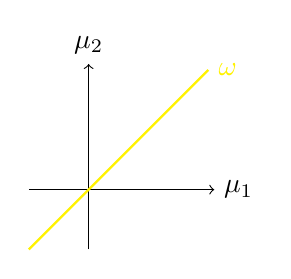
\begin{tikzpicture}[scale=0.38]
  \draw[->] (-2, 0) -- (4.2, 0) node[right] {$\mu_1$};
  \draw[->] (0, -2) -- (0, 4.2) node[above] {$\mu_2$};
	\draw [yellow,thick] (-2,-2) -- (4,4) node [right] {$\omega$};
\end{tikzpicture}
\end{minipage}
\end{frame}
%-------------- end slide -------------------------------%}}}
%-------------- start slide -------------------------------%{{{ 6.43
\begin{frame}
\begin{itemize}
	\item Let $Y_1,\cdots,Y_n$ be a random sample of size $n$ from $f_Y(y;\theta_1,\cdots,\theta_k)$\\[1em]
	\item Let $\Omega$ be all possible values of the parameter vector $(\theta_1,\cdots,\theta_k)$\\[1em]
	\item Let $\omega\subseteq \Omega$ be a subset of $\Omega$.
		\vfill
	\item Test:
		\[
			H_0: \theta\in\omega\quad\text{vs}\quad
			H_1: \theta\in\Omega\setminus\omega.
		\]
		\vfill
	\item The \textcolor{yellow!80!black}{\bf generalized likelihood ratio}, $\lambda$, is defined as
		\[
			\lambda := \frac{\displaystyle \max_{(\theta_1,\cdots,\theta_k)\in\omega} L(\theta_1,\cdots,\theta_k)}{\displaystyle \max_{(\theta_1,\cdots,\theta_k)\in \Omega}L(\theta_1,\cdots,\theta_k)}
		\]
\end{itemize}
\end{frame}
%-------------- end slide -------------------------------%}}}
%-------------- start slide -------------------------------%{{{ 6.44
\begin{frame}

\begin{itemize}
	\item[]
	\begin{align*}
		\lambda\in (\alert{0},\textcolor{green}{1}]
	\end{align*}
	\begin{center}
	% \begin{tabular}{ccc}
	%  $\lambda$ close to \alert{zero} & data are NOT compatible with $H_0$ & \alert{reject $H_0$}\\
	%  $\lambda$ close to \textcolor{green}{one} &  data are compatible with $H_0$ & \textcolor{green}{accept $H_0$}\\
	% \end{tabular}
\begin{minipage}{0.45\textwidth}
	\begin{center}
		$\lambda$ close to \alert{zero} \\
		data NOT compatible with $H_0$ \\
		\alert{reject $H_0$}
	\end{center}
\end{minipage}
\hfill
\begin{minipage}{0.45\textwidth}
	\begin{center}
		$\lambda$ close to \textcolor{green}{one} \\
		data compatible with $H_0$ \\
		\textcolor{green}{accept $H_0$}
	\end{center}
\end{minipage}
	\end{center}
		\vfill
	\item \textcolor{yellow!80!black}{\bf Generalized likelihood ratio test (GLRT)}: Use the following critical region
		\[
			C =\left\{\lambda: \lambda\in(0,\lambda^*]\right\}
		\]
		to reject $H_0$ with either $\alpha$ or $y^*$ being determined through
		\[
			\alpha = \bbP\left(0<\Lambda\le \lambda^*\bigg| \text{$H_0$ is true}\right).
		\]
\end{itemize}
\end{frame}
%-------------- end slide -------------------------------%}}}
%-------------- start slide -------------------------------%{{{ 6.45
\begin{frame}
	Remarks:\\[1em]
	\begin{enumerate}
		\item Maximization over $\Omega$ instead of $\Omega\setminus\omega$ in denominator:
		\item[]		In practice, little effect on this change.
		\item[]	In theory, much easier/nicer: $L(\theta_1,\cdots,\theta_k)$ is maximized over the whole space $\Omega$ by the max. likelihood estimates: $\Omega_e:=(\theta_{e,1},\cdots,\theta_{e,k})\in\Omega$.
			\vfill
		\item Suppose the maximization over $\omega$ is achieved at $\omega_e\in\omega$.
			\vfill
		\item Hence:
			\[
			\lambda = \frac{L(\omega_e)}{L(\Omega_e)}.
			\]
\end{enumerate}
\end{frame}
%-------------- end slide -------------------------------%}}}
%-------------- start slide -------------------------------%{{{ 6.46
\begin{frame}
	Remarks;\\[1em]
	\begin{enumerate}
	\setcounter{enumi}{3}
	\item For simple-vs-composite test, $\omega=\{\omega_0\}$ consists only one point: \\[1em]
			\[
		\lambda = \frac{L(\omega_0)}{L(\Omega_e)}.
			\]
		\vfill
	\item Working with $\Lambda$ is hard since $f_\Lambda(\lambda|H_0)$ is hard to obtain. \\[1em]
	\item[] If $\Lambda$ is a {\it (monotonic) function} of some r.v. $W$, whose pdf is known. \\[1em]
	\item[]
		\begin{center}
		Suggesting testing procedure \\[1em]
		Test based on $\lambda$
		$\quad\Longleftrightarrow\quad$
		Test based on $w$.
		\end{center}
	\end{enumerate}
\end{frame}
%-------------- end slide -------------------------------%}}}
%-------------- start slide -------------------------------%{{{ 6.47
\begin{frame}
	\begin{enumerate}
		\item[E.g. 1] Let $Y_1,\cdots,Y_n$ be a random sample of size $n$ from the uniform pdf: $f_Y(y:\theta)=1/\theta$, $y\in[0,\theta]$. Find the form of GLRT for
			\[
				H_0: \theta=\theta_0\quad\text{v.s.}
				\quad
				H_1:\theta<\theta_0
				\qquad\quad \text{with given $\alpha$.}
			\]
\vfill
\item[Sol.] 1) The null hypothesis is simple, and hence
	\[
		L(\omega_e) = L(\theta_0) = \theta_0^{-n} \prod_{i=1}^n I_{[0,\theta_0]}(y_i)
		=\theta^{-n}I_{[0,\theta_0]}(y_{max}).
	\]
\item[]	2) The MLE for $\theta$ is $y_{max}$ and hence,
	\[
		L(\Omega_e) = L(y_{max}) =
		y_{max}^{-n}I_{[0,y_{max}]}(y_{max})= y_{max}^{-n}.
	\]
	\end{enumerate}
\end{frame}
%-------------- end slide -------------------------------%}}}
%-------------- start slide -------------------------------%{{{ 6.48
\begin{frame}

	\begin{enumerate}
	\item[]	3) Hence,
		\[
			\lambda =
			\frac{L(\omega_e)}{L(\Omega_e)} =
			\left(\frac{y_{max}}{\theta_0}\right)^nI_{[0,\theta_0]}(y_{max})
		\]
	\item[] that is, the test statistic is
			\[
				\Lambda = \left(\frac{Y_{max}}{\theta_0}\right)^n I_{[0,\theta_0]}(Y_{max}).
			\]
			\vfill
	\item[] 4) $\alpha$ and critical value $\lambda^*$:
\begin{align*}
			\alpha & =
			\bbP(0<\Lambda\le \lambda^*| \text{$H_0$ is true})
			\\&=
			\bbP\left(\left[\frac{Y_{max}}{\theta_0}\right]^n I_{[0,\theta_0]}(Y_{max}) \le \lambda^*\bigg| \text{$H_0$ is true}\right)
			\\&=
			\bbP\left(Y_{max}  \le\theta_0 (\lambda^*)^{1/n}\bigg| \text{$H_0$ is true}\right)
		\end{align*}
		\vfill
	\item[] \hspace{2em} $\Lambda$ suggests the test statistic $Y_{max}$:\\[0.5em]
		\[\text{Test based on $\lambda$ $\Longleftrightarrow$ Test based of $y_{max}$}\]
	\end{enumerate}
\end{frame}
%-------------- end slide -------------------------------%}}}
%-------------- start slide -------------------------------%{{{ 6.49
\begin{frame}
	\begin{enumerate}
		\item[] 5) Let's find the pdf of $Y_{max}$. The cdf of $Y$ is $F_Y(y;\theta_0) = y/\theta_0$ for $y\in [0,\theta_0]$. Hence,
			\begin{align*}
				f_{Y_{max}}(y;\theta_0)
				&=n F_Y(y;\theta_0)^{n-1}f_Y(y;\theta_0)\\
				&= \frac{n y^{n-1}}{\theta_0^n},\quad y\in [0,\theta_0].
			\end{align*}
			\vfill
		\item[] 6) Finally, by setting $y^*:= \theta_0(\lambda^*)^{1/n}$, we see that
			\begin{align*}
				\alpha&=
				\bbP\left(Y_{max}  \le y^* \bigg| \text{$H_0$ is true}\right)
				    \\&= \int_0^{y^*} \frac{ny^{n-1}}{\theta_0^n} \ud y
				    \\&= \frac{(y^*)^n}{\theta_0^n} \quad\Longleftrightarrow\quad
				    y^* = \theta_0 \alpha^{1/n}.
			\end{align*}
			\vfill
		\item[]	7) Therefore, $H_0$ is rejected if
			\[
				y_{max}\le  \theta_0 \alpha^{1/n}.
			\]
			\myEnd
	\end{enumerate}
\end{frame}
%-------------- end slide -------------------------------%}}}
%-------------- start slide -------------------------------%{{{ 6.50 Eg. 2
\begin{frame}

	\begin{enumerate}
		\item[E.g. 2] Let $X_1,\cdots,X_n$ be a random sample from the geometric distribution with parameter $p$.
			% \[
				% p_X(k;p) = (1-p)^{k-1}p, \quad k=1,2,\cdots
			% \]
		\item[] Find a test statistic $\Lambda$ for testing
			$H_0 : p = p_0$ versus $H_1 : p \ne p_0$.
			\vfill
		\item[Sol.] Let $\overline{X}$ and $\overline{k}$ be the sample mean. Because the null hypothesis is simple,
	\[
		L(\omega_e) = L(p_0) =  \prod_{i=1}^n  (1-p_0)^{k_i-1}p_0= (1-p_0)^{n \bar{k}-n} p_0^n,
	\]
\item[] which shows that $\bar{k}$ is a sufficient estimator.
\item[] On the other hand, the MLE for the parameter $p$ is $1/\bar{k}$. So
	\[
		L(\Omega_e) = L(1/\bar{k}) = \prod_{i=1}^n \left(1-\frac{1}{\bar{k}}\right)^{k_i-1}\frac{1}{\bar{k}} = \left(\frac{\bar{k}-1}{\bar{k}}\right)^{n\bar{k}-n} \frac{1}{\bar{k}^{n}}.
	\]
\item[]	Hence,
	 \[\lambda=\frac{L(\omega_e)}{L(\Omega_e)}
	 = \left(\frac{\bar{k}(1-p_0)}{\bar{k}-1}\right)^{n\bar{k}-n} (p_0 \bar{k})^n\]
 \item[] Finally, $\Lambda= \left(\frac{\overline{X}(1-p_0)}{\overline{X}-1}\right)^{n\overline{X}-n} (p_0 \overline{X})^n$. \myEnd
	\end{enumerate}
\end{frame}
%-------------- end slide -------------------------------%}}}
%-------------- start slide -------------------------------%{{{ 6.51 Eg 3
\begin{frame}

\begin{enumerate}
		\item[E.g. 3] Let $Y_1,\cdots,Y_n$ be a random sample from the exponential distribution with parameter $\lambda$.
		\item[] Find a test statistic $V$ for testing $H_0 : \lambda = \lambda_0$ versus $H_1 : \lambda \ne \lambda_0$.
			\vfill
		\item[Sol.]Since the null hypothesis is simple,
			\[
				L(\omega_e) = L(\lambda_0)  = \prod_{i=1}^n \lambda_0e^{-\lambda_0 y_i} = \lambda_0^n e^{-\lambda_0 \sum_{i=1}^n y_i}
			\]
		\item[] Let $Z=\sum_{i=1}^n Y_i\sim$ Gamma$(n,\lambda)$, which is a sufficient estimator.
		\item[] On the other hand, the MLE for $\lambda$ is $1/\bar{y}=n/z$:
			\[
				L(\Omega_e) = L(1/\bar{y}) = (n/z)^{n} e^{-n}.
			\]
	 \item[] Hence,
		 \[
			 \lambda =\frac{L(\omega_e)}{L(\Omega_e)} = z^nn^{-n} \lambda_0^n e^{-\lambda_0 z+n}
		 \]
 \item[] Finally, $\Lambda=Z^nn^{-n} \lambda_0^n e^{-\lambda_0 Z+n} $\qquad \pause or \qquad $V = Z^n e^{-\lambda_0 Z}$. \myEnd
	\end{enumerate}
\end{frame}
%-------------- end slide -------------------------------%}}}
%-------------- start slide -------------------------------%{{{ 1
\begin{frame}[fragile]
\begin{itemize}
	\item[] The critical region in terms of $V$ should be:
	\begin{align*}
		0.05 = \alpha & = \bbP\left(V\in(0,y^*]\bigg|\text{$H_0$ is true}\right)\\
		& = \int_0^{y^*} f_V(v)\ud v
	\end{align*}
	\item[] However, it is not easy to find the exact distribution of $V$.
	\vfill
	\item[] One can also make the inference based on the test statistic $Z$ ...
	\end{itemize}
\end{frame}
%-------------- end slide -------------------------------%}}}
%-------------- start slide -------------------------------%{{{ 1 v(z) function plot
\begin{frame}[fragile]
\begin{center}
	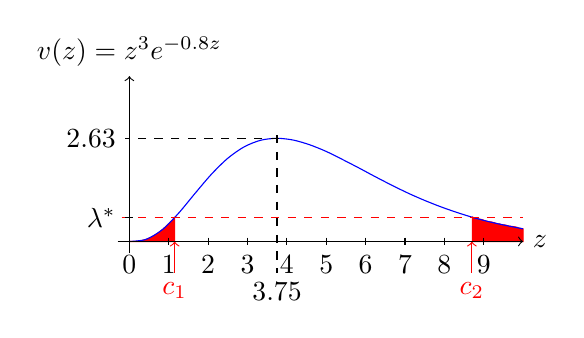
\begin{tikzpicture}[scale=0.5]
  % \filldraw[scale=1, domain=3.7:3.8, smooth, variable=\x, green] plot ({\x}, {\x*\x*\x*exp(-0.8*\x)}) -- (3.8,2.6248) -- (3.7,2.6248);
	\def\left{1.15}
  \filldraw[scale=1, domain=0:\left, smooth, variable=\x, red] plot ({\x}, {\x*\x*\x*exp(-0.8*\x)}) -- (\left,0) -- (0,0);
	\def\right{8.7}
  \filldraw[scale=1, domain=\right:10, smooth, variable=\x, red] plot ({\x}, {\x*\x*\x*exp(-0.8*\x)}) -- (10,0) -- (\right,0);
  \draw[scale=1, domain=0:10, smooth, variable=\x, blue] plot ({\x}, {\x*\x*\x*exp(-0.8*\x)});
	\foreach \x in {0,...,9}{
			\draw (\x,0.1)--++(0,-0.2) node [below] {$\x$};
	}
	\draw[dashed] (3.75,2.7) -- (3.75,-0.8) node [below] {$3.75$};
	\draw[dashed] (3.8,2.6255) -- (-0.1,2.6255) node [left] {$2.63$};
	\def\level{0.6}
	\draw[dashed,red] (-0.2,\level) -- (10,\level);
	\draw[red,<-] (\left,0) -- (\left, -0.8) node [below] {$c_1$};
	\draw[red,<-] (\right,0) -- (\right, -0.8) node [below] {$c_2$};
	\draw (-0.1,\level) node [left] {$\lambda^*$} -- (0.1,\level);
  \draw[->] (-0.3, 0) -- (10, 0) node[right] {$z$};
  \draw[->] (0, -0.3) -- (0, 4.2) node[above] {$v(z)=z^3e^{-0.8z}$};
	\end{tikzpicture}

	\vfill

	This suggests that the critical region in terms of $z$ should be of the form:
	\begin{align*}
		(0,c_1) \cup (c_2,\infty)
	\end{align*}
	For convenience, we put $\alpha/2$ mass on each tails of the density of $Z$:\\[1em]
	Find $c_1$ and $c_2$ such that
	\begin{align*}
		\int_0^{c_1} f_{Z}(z)dz = \int_{c_2}^\infty f_{Z}(z)dz = \frac{\alpha}{2}.
	\end{align*}
\end{center}
\end{frame}
%-------------- end slide -------------------------------%}}}
%-------------- start slide -------------------------------%{{{ 1
\begin{frame}[fragile]
\begin{center}

	\renewcommand{\arraystretch}{2}
	\begin{tabular}{c|cc}
                  & using $V$      & using $Z$                  \\ \hline
	Critical region & $(0,v^*]$      & $(0,z_1]\cup [z_2,\infty)$ \\
	pdf             & hard to obtain & Gamma $(n,\lambda)$        \\
	\end{tabular}
\end{center}
\end{frame}
%-------------- end slide -------------------------------%}}}
%-------------- start slide -------------------------------%{{{ 6.52 Eg. 4
\begin{frame}

	\begin{enumerate}
		\item[E.g. 4] Let $Y_1,\cdots,Y_n$ be a random sample from $N(\mu,1)$.
		\item[] Find a test statistic $\Lambda$ for testing $H_0 : \mu = \mu_0$ versus $H_1 : \mu \ne \mu_0$.
			\vfill
		\item[Sol.]Since the null hypothesis is simple,
\[
	L(\omega_e) = L(\mu_0) = \prod_{i=1}^n\frac{1}{\sqrt{2\pi}}e^{-\frac{(y_i-\mu_0)^2}{2}}.
\]
\item[] On the other hand, the MLE for $\mu$ is $\bar{y}$:
	\[
	L(\Omega_e) = L(\bar{y}) =
	\prod_{i=1}^n\frac{1}{\sqrt{2\pi}}e^{-\frac{(y_i-\bar{y})^2}{2}}.
	\]
\item[] Hence,
\[	 \lambda=\frac{L(\omega_e)}{L(\Omega_e)}
	 = \exp\left(-\sum_{i=1}^n \frac{(y_i-\mu_0)^2 -(y_i-\bar{y})^2}{2}\right)
	 = \exp\left(-\frac{n (\bar{y}-\mu_0)^2}{2}\right).
\]
 \item[] Finally, $\Lambda= \exp\left(-\frac{n}{2} \left(\overline{Y}-\mu_0\right)^2
	 \right)$\pause\qquad or\qquad $V =  \frac{\overline{Y}-\mu_0}{1/\sqrt{n}}\sim N(0,1)$ \myEnd
	\end{enumerate}
\end{frame}
%-------------- end slide -------------------------------%}}}
